\documentclass[conference]{IEEEtran}
\usepackage{graphicx}
\usepackage{epstopdf}
\usepackage[utf8]{inputenc}
\usepackage{amsmath, amsfonts, amssymb}
\usepackage{float}
\usepackage[portuguese]{babel}
\usepackage {hyperref}
\usepackage{indentfirst}
\usepackage{placeins}
\usepackage[]{algorithm2e}
\usepackage{setspace}
\usepackage{color}
\renewcommand{\rmdefault}{ptm}
\setlength{\parindent}{1cm} 

\newcommand{\Fix}[1]{\textbf{[[}{\color{red} #1}\textbf{]]}}
\newcommand{\Anonim}[2]{#1}
\newcommand{\ie}{i.e.}
\newcommand{\eg}{e.g.}
\newcommand{\cf}{cf.}
\newcommand{\etal}{et al.}

\definecolor{bs}{rgb}{0.59, 0.0, 0.09}

\newcommand{\Davino}[1]{\textbf{[Davino:[}{\color{bs} #1}\textbf{]]}}
\newcommand{\Victor}[1]{\textbf{[Victor:[}{\color{bs} #1}\textbf{]]}}

\newcommand{\cmark}{\ding{51}}%
\newcommand{\xmark}{\ding{55}}%


\begin{document}

\title{Improving QoS in Vehicular ad-hoc Networks using a Multi-Objective Genetic Algorithm}

\author{\IEEEauthorblockN{Davino Mauro Tenório da Silva Júnior}
\IEEEauthorblockA{Centro de Informática\\
Universidade Federal de Pernambuco\\
Email: dmtsj@cin.ufpe.br}
\and
\IEEEauthorblockN{Victor Hugo Sabino dos Santos Aráujo}
\IEEEauthorblockA{Centro de Informática\\
Universidade Federal de Pernambuco\\
Email: vhssa@cin.ufpe.br}}

\maketitle

\begin{abstract}
As rápidas mudanças de topologia em Redes \textit{Ad-Hoc} Veiculares (VANETs) são comuns devido a grande mobilidade dos nós. Para obter uma transmissão de pacotes eficiente, é preciso avaliar os parâmetros de rede, e encontrar um valor ótimo de acordo com a rede e condições de tráfego. Neste artigo, é apresentado um esquema de otimização Multiobjetiva utilizando o algoritmo \textit{Fast Non-Dominated Sorting Algorithm} (NSGA-II) para melhorar a Qualidade de Serviço (QoS) em redes VANET.
\\
\\
Palavras Chave: VANETs, QoS, NSGA-II, Perda de Pacotes, Delay, Throughput.
\end{abstract}

\section{Introdução}

Os Sistemas de Transporte Inteligentes (ITS), de acordo com ~\cite{Vanajakshi:2010}, lidam com as questões de tráfego como congestionamento e disseminação de informações, e estão cada vez mais em destaque com o avanço das tecnologias de comunicação sem fio e de automóveis. As Redes \textit{Ad-Hoc} Veiculares (VANETs), que derivam das redes \textit{Ad-Hoc} Móveis (MANETs), permitem que veículos em movimento estejam conectados e se comuniquem sem fio. Esta comunicação pode ser entre dois veículos (V2V) ou entre um veículo e uma infraestrutura (V2I) ~\cite{Anwer:2016}.

Para estabelecer uma comunicação segura e eficiente entre veículos, é necessário que haja uma infraestrutura de comunicação adequada. O padrão IEEE 802.11p apresentado em ~\cite{Jiang:2008} de Comunicação Dedicada de Curto Alcance (DSRC) foi desenvolvido especificamente para requisitos das VANETs como: auto-organização, configuração automática, topologia dinâmica e alta mobilidade.

Para que a comunicação sem fio opere em tempo real, existem restrições associadas que precisam ser gerenciadas na camada física, como: o tempo de disseminação de dados (\textit{delay}), a perda de pacotes e a taxa de transferência (\textit{throughput}). ~\cite{Dai:2016} diz que para garantir um desempenho otimizado em tempo real, é necessário que ambas as restrições sejam atendidas simultaneamente, o que não é trivial devido à limitação de banda e o ambiente veicular altamente dinâmico.

Dentre os vários desafios de VANETs abordados na literatura, ~\cite{Cunha:2017} destaca o cenário dinâmico e a necessidade de protocolos específicos para redes veiculares que sejam menos afetados pelas frequentes mudanças na rede. ~\cite{Lim:2015} aponta o problema de terminal escondido como a principal causa de perda de pacotes em VANETs e propõe uma solução de otimização adaptativa baseada em lógica \textit{Fuzzy} para resolvê-lo. Já ~\cite{Almohammedi:2016} faz uma análise do impacto do alcance de trasmissão no desempenho de VANETs em termos de taxa de entrega de pacotes e delay, enquanto ~\cite{Rawat:2011} relaciona a potência de transmissão de acordo com seu alcance. ~\cite{Lim:2015} também destaca a importância de uma janela de contenção dinâmica, que seja otimizada de acordo com o congestionamento no canal. ~\cite{Schmidt:2009} mostra que a interferência é um dos principais fatores da degradação de transmissão em VANETs, a qualidade do sinal pode ser calculada através da SINR, que é considerado um bom indicador das condições de rede. Por isso, SINR será utilizado como parâmetro juntamente com a potência de transmissão e o tamanho da janela de contenção.

As principais contribuições deste artigo são: primeiramente, simular um cenário real de nós em movimento para extrair informações da rede como: \textit{delay}, perda de pacote e \textit{throughput}. Em seguida, definir um espaço amostral de parâmetros de entrada para a simulação, tendo como variáveis a potência de transmissão, o tamanho da janela de contenção ($CW_{min}$ e $CW_{max}$) e a Relação Sinal-Ruído mais Interferência (SINR). Com isso, é possível fazer uma simulação exaustiva com todo o espaço amostral e realizar um estudo comparativo com o resultado obtido através da aplicação de uma técnica de otimização baseada no algoritmo genético multi-objetivo \textit{Fast Non-dominated Sorting Algorithm} (NSGA-II).

O restante do artigo está organizado da seguinte forma: na Seção II, é apresentado o modelo do sistema a ser simulado; na Seção III, é formulado o problema multi-objetivo e apresentado o algoritmo NSGA-II; na Seção IV, é construído o modelo de simulação e a avaliação de seu desempenho; a seção V conclui o trabalho e são discutidos possíveis trabalhos futuros.

\section{Modelo do Sistema}

Neste estudo, é considerado um ambiente urbano comumente encontrado em regiões metropolitanas. O cenário utilizado para a simulação foi retirado do \textit{OpenStreetMaps}, o ambiente é localizado no centro da cidade do Recife, nas mediações da Av. Agamenom Magalhães. O número de veículos dentro da rede aumenta conforme o tempo de simulação, e são aleatoriamente colocados no mapa e com velocidade variando de acordo com o tráfego do local, tornando o modelo mais realista. %%\textbf{[precisamos saber como foi a simulação do sumo para inserir detalhes e uma imagem do mapa aqui, a figura abaixo seria aquele cenário dos carros se movimentando que foi mostrado em sala.]}


%%\begin{figure}[t]
 %% \centering
  %%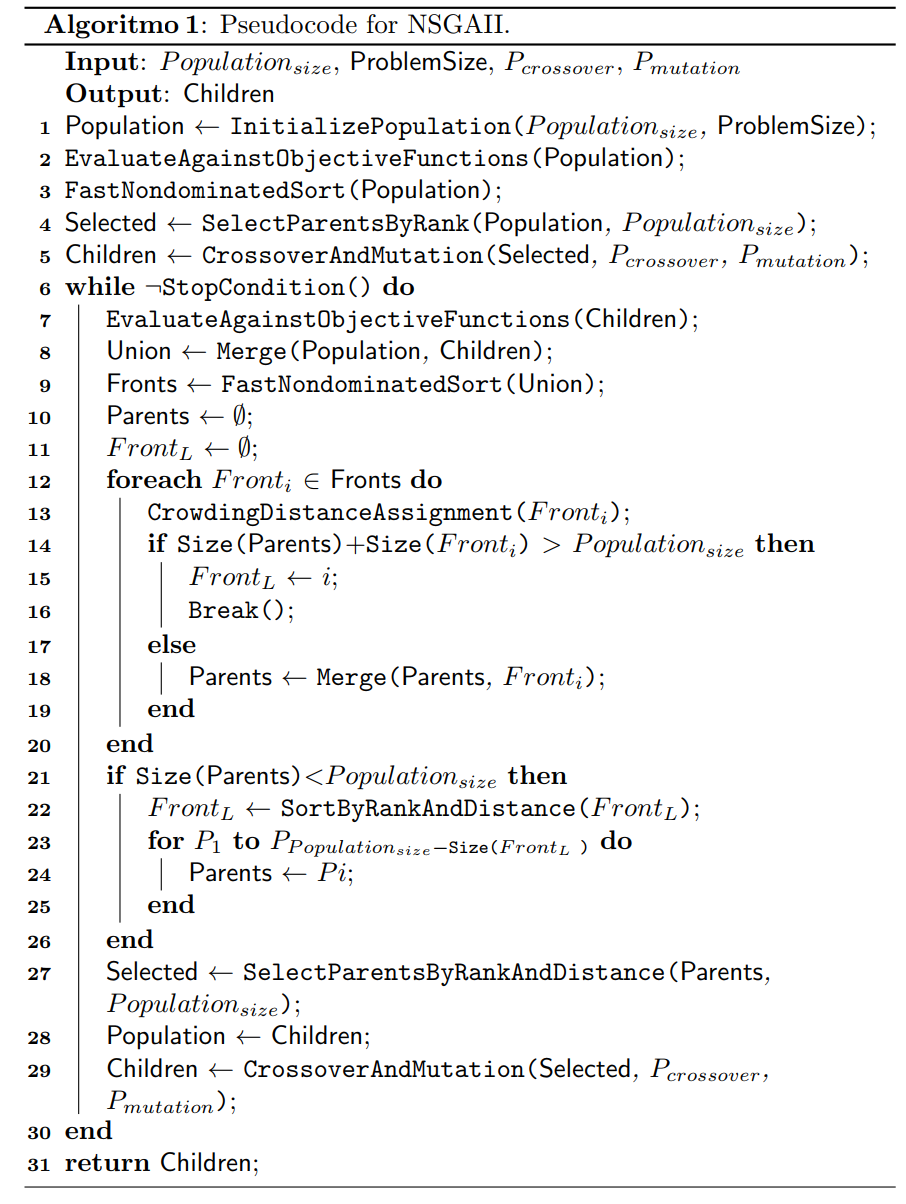
\includegraphics[scale=0.4]{figures/pseudocodigo.png}
  %%\caption{Fragmento da cidade do Recife utilizado no cenário}
  %%\label{fig:how_pop3_works}
%%\end{figure}

Assume-se que todos os veículos estão equipados com uma Unidade de Controle de Bordo (OBU), que dá suporte a comunicações V2I e V2V. Adicionalmente, os veículos são capazes de transmitir e receber informações atualizadas enquanto trafegam sobre o tráfego, acidentes, e informações baseadas em localização.

\section{Formulação do Problema}
\label{sec:form-problema}

Baseado nas informações anteriores, o objetivo deste estudo é minimizar a perda de pacotes e o \textit{delay} de disseminação, e aumentar o \textit{throughput} de dados de uma rede VANET considerando apenas a comunicação entre veículos (V2V). Portanto, pode-se propor uma técnica de Otimização Multi-Objetiva (MOO) para resolver este problema. A MOO é um campo que diz respeito a otimização de duas ou mais funções objetivas ~\cite{Brownlee:2011}. A solução deste problema envolve a localização de um conjunto de soluções candidatas chamadas de não dominadas. O conjunto de soluções não dominadas ótimas é chamado de pareto ótimo. Todas as soluções que estão no pareto ótimo pertencem ao conjunto de paretos, e os pontos representados em relação a cada objetivo no espaço são chamados de pareto \textit{front}. A complexidade dos problemas MOO são diretamente ligadas as dependências entre as variáveis de decisão em relação a seus objetivos, no caso em que existem conflitos entre estas variáveis, é necessário um \textit{trade-off} para analisar qual objetivo deve ser priorizado.

O presente trabalho adotou o algoritmo genético multiobjetivo denominado \textit{Fast Non-dominated Sorting Genetic Altorithm} (NSGA-II) proposto por ~\cite{Deb:2002}. Este algoritmo aplica o conceito de dominância ao classificar elementos da população de maneira elitista em fronteiras (\textit{fronts}), de acordo com o grau de dominância. A cada geração, os indivíduos classificados no primeiro \textit{front} são considerados melhores, ou, dominantes. Após a classificação em \textit{fronts}, os indivíduos também são ordenados através de um operador de diversidade baseado num indicador de densidade (\textit{crowding distance}), que relaciona a distância de cada indivíduo para seus vizinhos imediatos com a distância entre as soluções extremas do mesmo \textit{front}. O pseudocódigo para o NSGA-II é apresentado no Algoritmo 1 a seguir. A função \textit{SortByRankAndDistance} ordena a população em uma hierarquia de Pareto \textit{fronts} não dominados, já a \textit{CrowdingDistanceAssignment} calcula a distância média entre membros de cada front. Já a função \textit{CrossoverAndMutation} executa as operações de mutação e cruzamento do GA. Já as funções \textit{SelectParentsByRankAndDistance} e \textit{SortByRankAndDistance} fazem a seleção dos membros da população em termos de precedência do front a qual a solução pertence, e a distância dele para o front, calculado anteriormente pelo \textit{CrowdingDistanceAssignment}.

\begin{figure}[t]
 %% \centering
  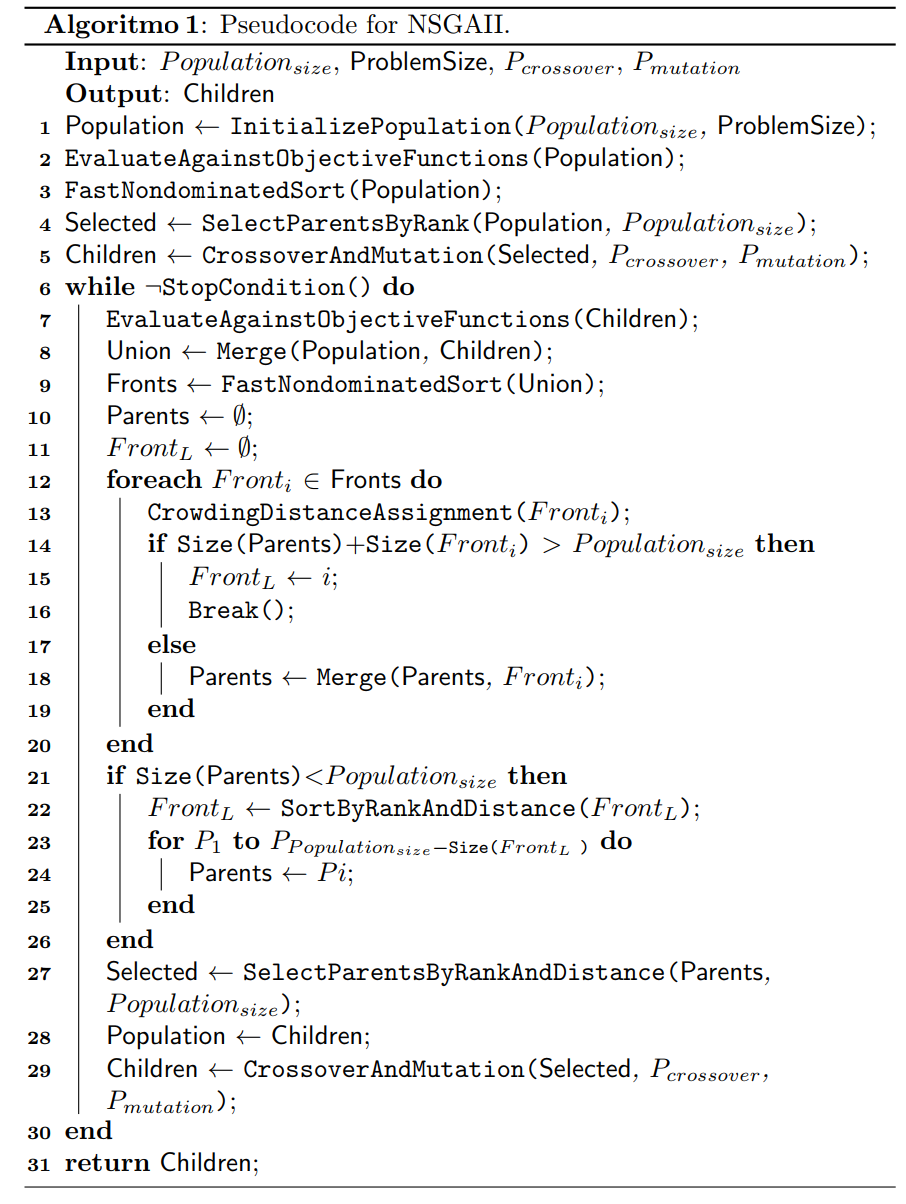
\includegraphics[scale=0.37]{figures/pseudocodigo.png}
  %%\caption{Fragmento da cidade do Recife utilizado no cenário}
  %%\label{fig:how_pop3_works}
\end{figure}


\section{Avaliação do desempenho}
\label{sec:avaliacao-desemp}

Neste trabalho, os cenários descritos na seção ~\ref{sec:form-problema} foram simulados utilizando a ferramenta \textit{Vehicles in Network Simulation} (VEINS), que é composto de dois simuladores, o OMNeT++, que é um simulador de redes baseado em eventos e o \textit{Simulation of Urban Mobility} (SUMO) para simulação de tráfego em estradas, que pode extrair rotas do mundo real através do banco de dados do OpenStreetMap [12]. Ambos os simuladores são gratuitos e dispõe de tutoriais para os interessados em aprender a utilizá-los. A simulação no VEINS foi realizada de forma exaustiva, dados os parâmetros de configuração que serão descritos a seguir, e foi gerado  um arquivo de resultados. Para avaliação do algoritmo multi-objetivo em busca da melhor configuração de parâmetros a serem utilizados no simulador, foi utilizada uma implementação em Ruby do algoritmo NSGA-II com funções objetivo adaptadas para o problema proposto. As funções foram baseadas no problema multi-objetivo introduzido por Schaffer e apresentado em ~\cite{Deb:2001}, e visam maximizar o \textit{throughput} e minimizar a perda de pacotes e \textit{delay}.

Foi utilizada uma implementação do algoritmo NSGA-II na linguagem de programação Ruby ~\cite{Brownlee:2011}, adaptando a mesma para o problema e proposito deste trabalho.

\subsection{Parâmetros de Configuração}
\label{subsec:param-config}

Os parâmetros de configuração definidos foram a Potência de Transmissão (\textit{txpower}), a SINR (\textit{slotlength}), e o tamanho da janela de contenção ($CW_{min}$ e $CW_{max}$). Para avaliar o desempenho do NSGA-II em relação ao exaustivo, foi definido um conjunto de valores que compõe o espaço de busca, e ele está disposto da seguinte forma: \textit{txpower} = [1, 4, 6, 10, 12, 14, 17, 20, 24, 27, 29, 31, 32] $dBm$; $CW_{min}$ = [16, 32, 64, 128, 256, 512] \textit{bits}; $CW_{max}$ = [1024, 2048, 4096] \textit{bits}; \textit{slotlength} =  [5, 10, 15, 20, 25, 30, 35, 40, 45, 50, 55, 60, 65, 70, 75, 80, 85, 90, 95, 100] $\mu S$. Assim, o espaço de busca é de 4680 possibilidades ou simulações, considerando que o tempo para executar uma simulação seja de 600 segundos, o tempo necessário para simular todo o espaço é de 780 horas, pouco mais de um mês. Logo, a utilização de uma técnica de otimização pode reduzir o tempo de simulação e alcançar um resultado próximo do ótimo mais rapidamente.

\subsection{Simulação}

A representação do indivíduo no algoritmo NSGA-II se dá por um mapa de 16 bits.  Cada indivíduo é dividido de forma a representar os quatro parâmetros de configuração utilizados no simulador e descritos na seção ~\ref{subsec:param-config}, a saber (1) $CW_{min}$, (2) $CW_{max}$, (3) slot length, e (4) txPower, como mostra a figura ~\ref{fig:bits-config}.  A simulação consiste em efetuar o \textit{parse} desse indivíduo para uma dada configuracão, isto é, um valor para cada parãmetro, e buscar essa configuração no arquivo resultante da busca exaustiva. Uma vez encontrados os resultados da simulação realizada com os parâmetros de configuração do indivíduo,
isto é, \textit{throughput}, perda de pacotes e \textit{delay}, são calculadas as respectivas funções objetivo buscando determinar se o indivíduo é ótimo, isto é, se condizem com os objetivos propostos na seção ~\ref{sec:avaliacao-desemp}. O algoritmo NSGA-II busca então pelo pareto \textit{front} com os melhores resultados de simulação para um dado indivíduo (configuração), executando o rankeamento dos paretos não dominados, e os passos de reprodução e \textit{crossover}.

Como função \textit{fictness}, ou função objetivo, foi adaptado a função de Shaffer, como mostra a figura ~\ref{fig:function}.
Para o algoritmo, Foi utilizada uma taxa de \textit{crossover} de 0.98\% e mutação ponto a ponto (\textit{bitstring}), como apresentado em [9].

\begin{figure}[t]
  \centering
  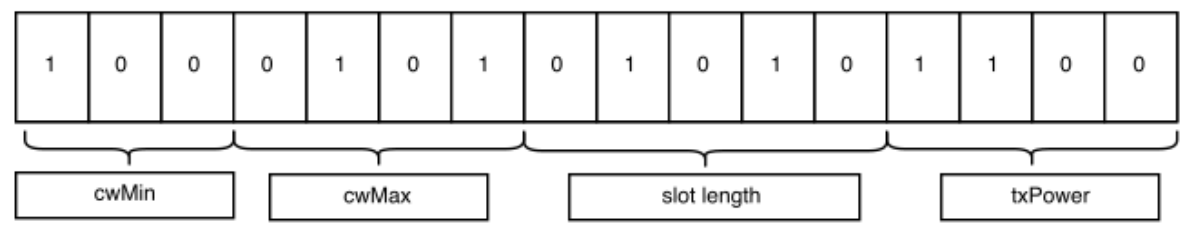
\includegraphics[scale=0.26]{figures/bits-config.png}
  \caption{Função \textit{fitness} utilizada. A variável X encontra-se num intervalo fechado de -10 a 10.}
  \label{fig:function}
\end{figure}


\begin{figure}[t]
  \centering
  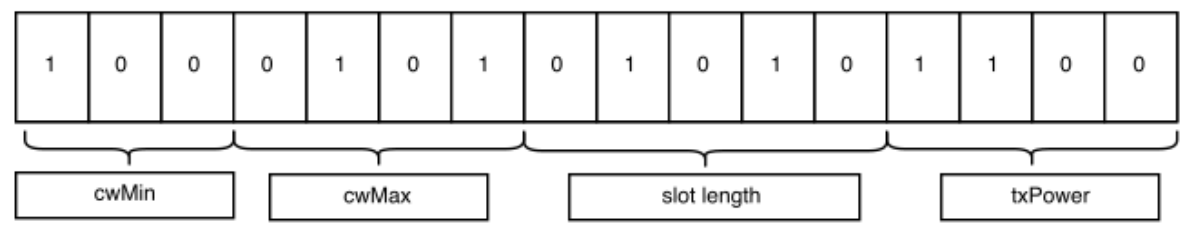
\includegraphics[scale=0.26]{figures/bits-config.png}
  \caption{Indivíduo utilizado no algoritmo representando uma possível configuração para simulação.}
  \label{fig:bits-config}
\end{figure}


\section{Resultados}

Para execução do algoritmo NSGA-II, foram utilizadas 50 gerações.
A população utilizada variou de 5 a 50, incrementando de 5 em 5. Os resultados em termos de \textit{throughput}, perda de pacotes e \textit{delay}
podem ser encontrados nas figuras ~\ref{fig:result-throughput},~\ref{fig:result-perda} e ~\ref{fig:result-delay}.

Em termos de \textit{throughput}, pode-se observar que os resultados convergem rapidamente, logo a partir das primeiras gerações, com poucas ocorrências de \textit{outliers} (como visto na 35 geração).
Pode-se observar também que, uma população menor que 30 indíviduos não apresenta convergência ou mesmo resultados ótimos. É importante notar que utiliza-se $throughput^{-1}$ em virtude dos valores simulados do \textit{throughput} serem muito baixos.

Em termos de perda de pacotes, os resultados convergem a partir de 35 gerações. Nota-se que, com uma população abaixo de 50 indivíduos, ocorre uma alta taxa de variação de resultados, sugerindo que populações com mais indivíduos podem ser utilizadas a fim de minimizar a perda de pacotes.

Em termos de \textit{delay}, populações acima de 40 indivíduos obtém resultados convergentes logo de início, o que sugere a otimização do algoritmo NSGA-II em obter resultados ótimos.
Populações abaixo de 40 indivíduos mostraram-se ineficazes em minimizar o \textit{delay}.

\begin{figure}[t]
  \centering
  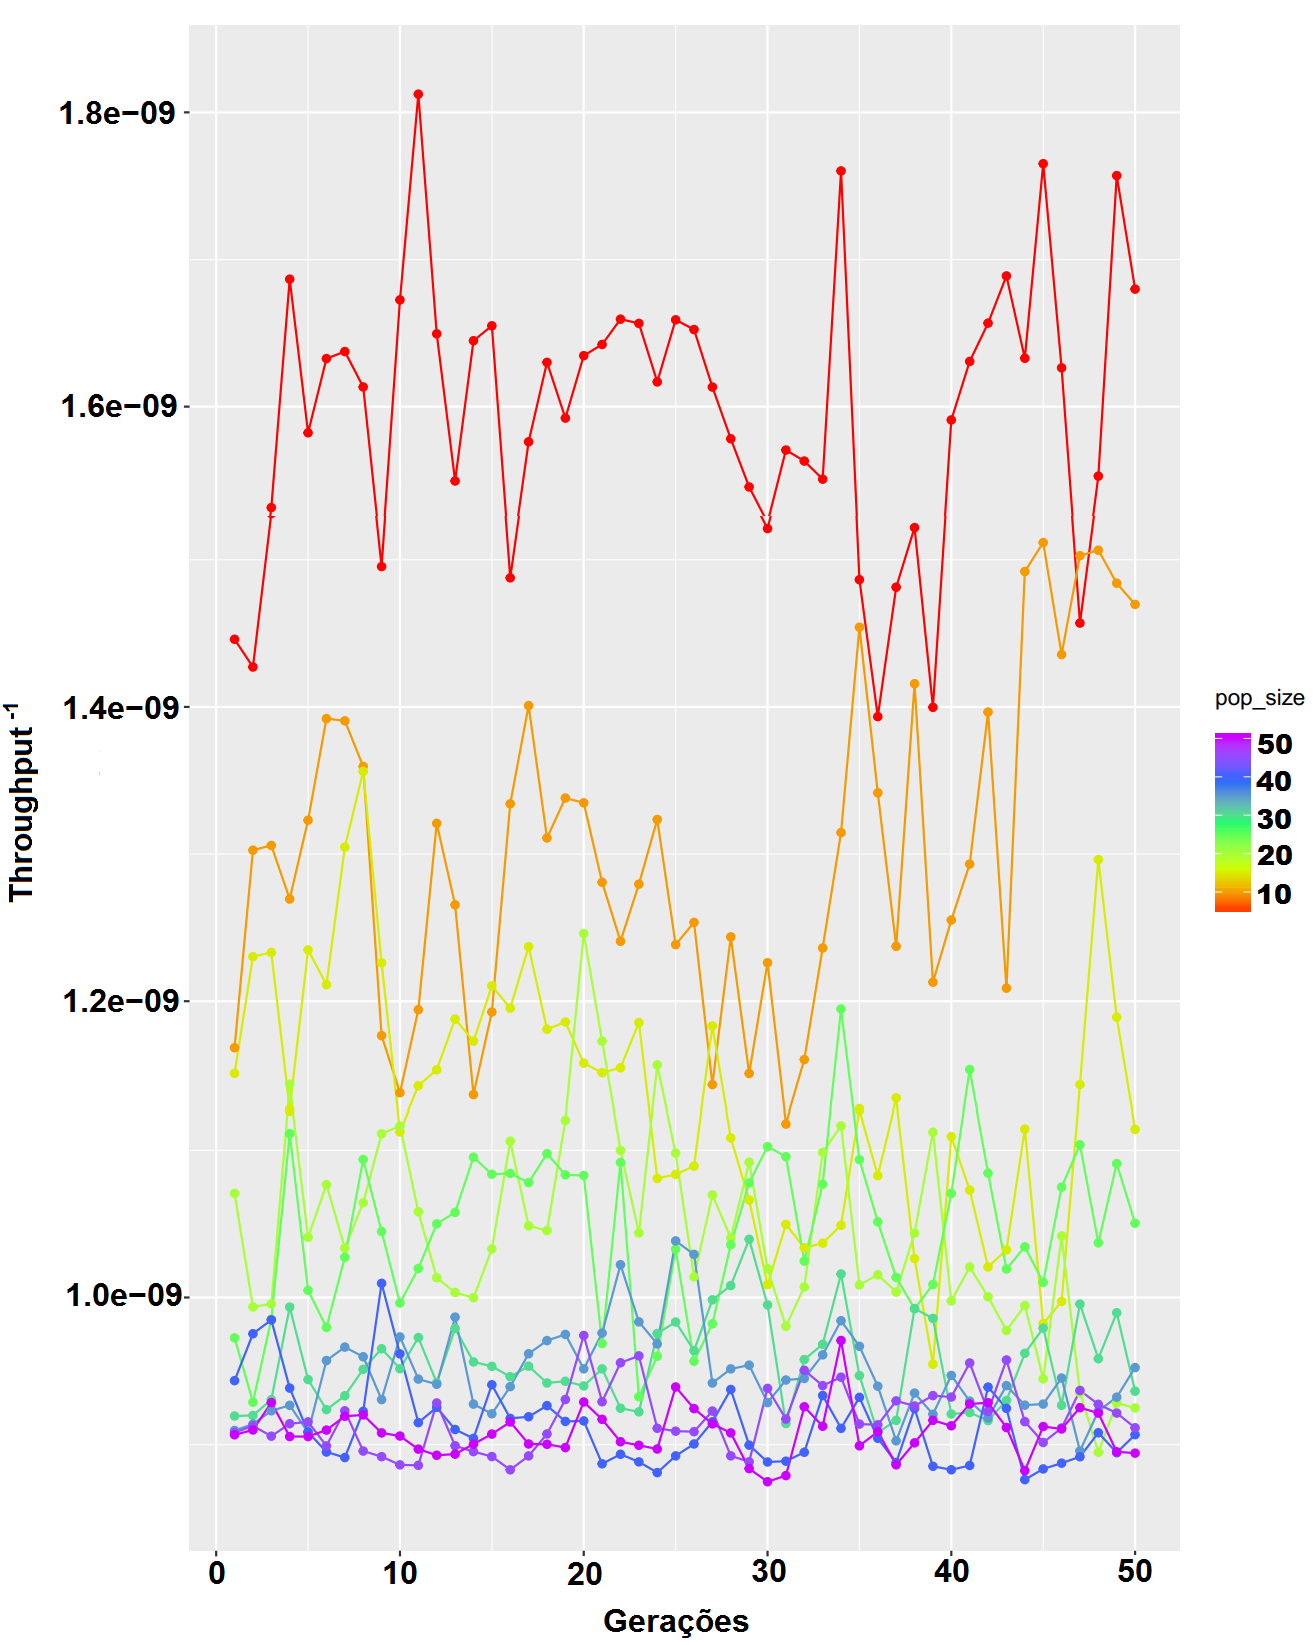
\includegraphics[scale=0.24]{figures/GeracoesXThroughput.png}
  \caption{Resultado em termos de gerações por média de 1/Throughput alcançados nas simulações.}
  \label{fig:result-throughput}
\end{figure}

\begin{figure}[t]
  \centering
  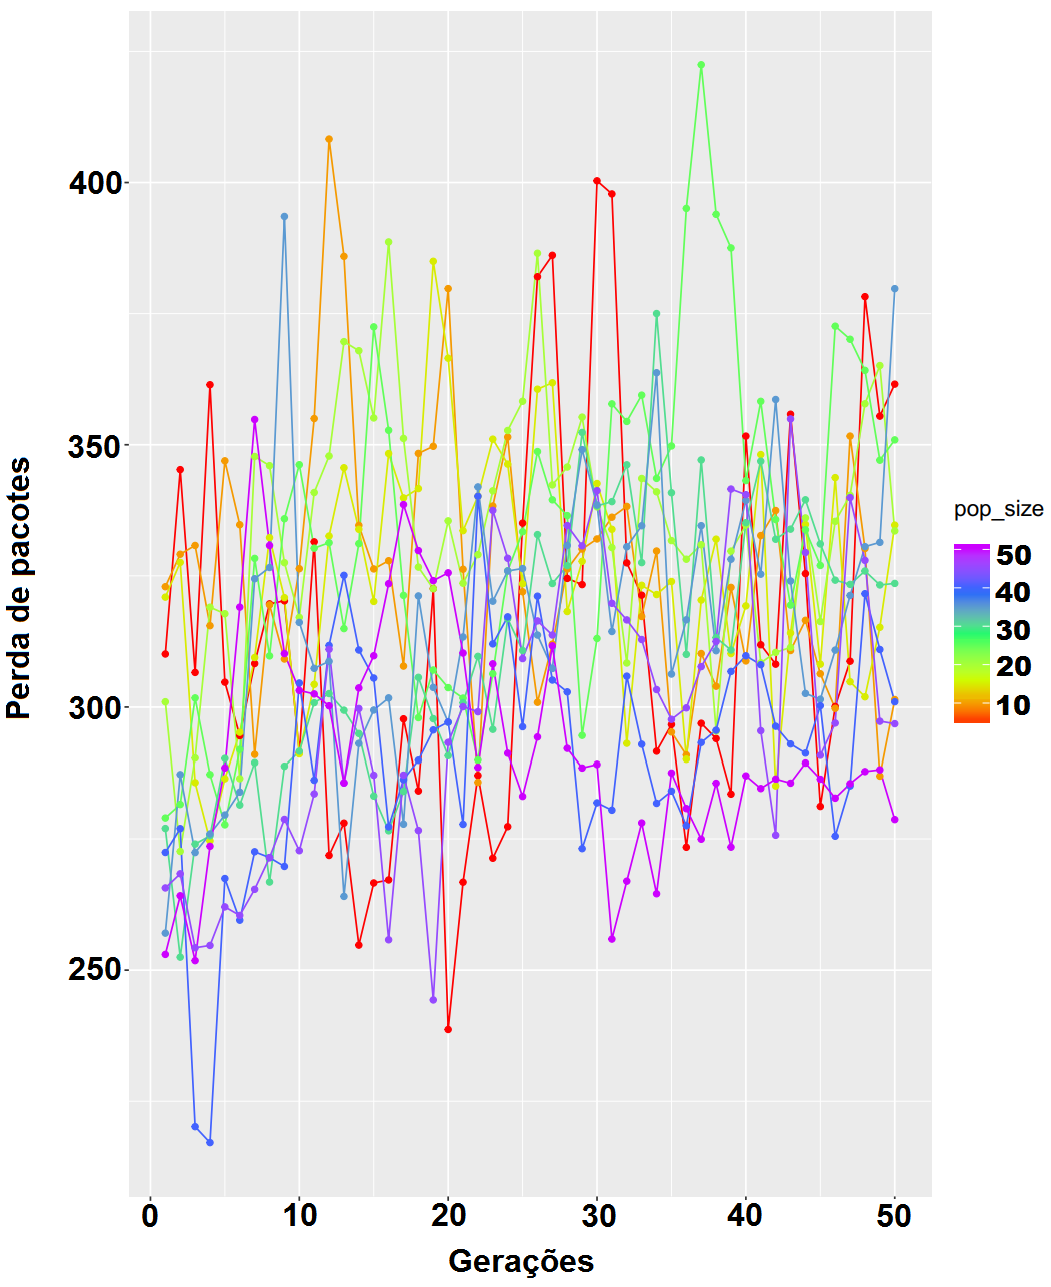
\includegraphics[scale=0.24]{figures/GeracoesXPerdaPacotes.png}
  \caption{Resultado em termos de gerações por média de perda de pacotes alcançados nas simulações.}
  \label{fig:result-perda}
\end{figure}


\begin{figure}[h]
  \centering
  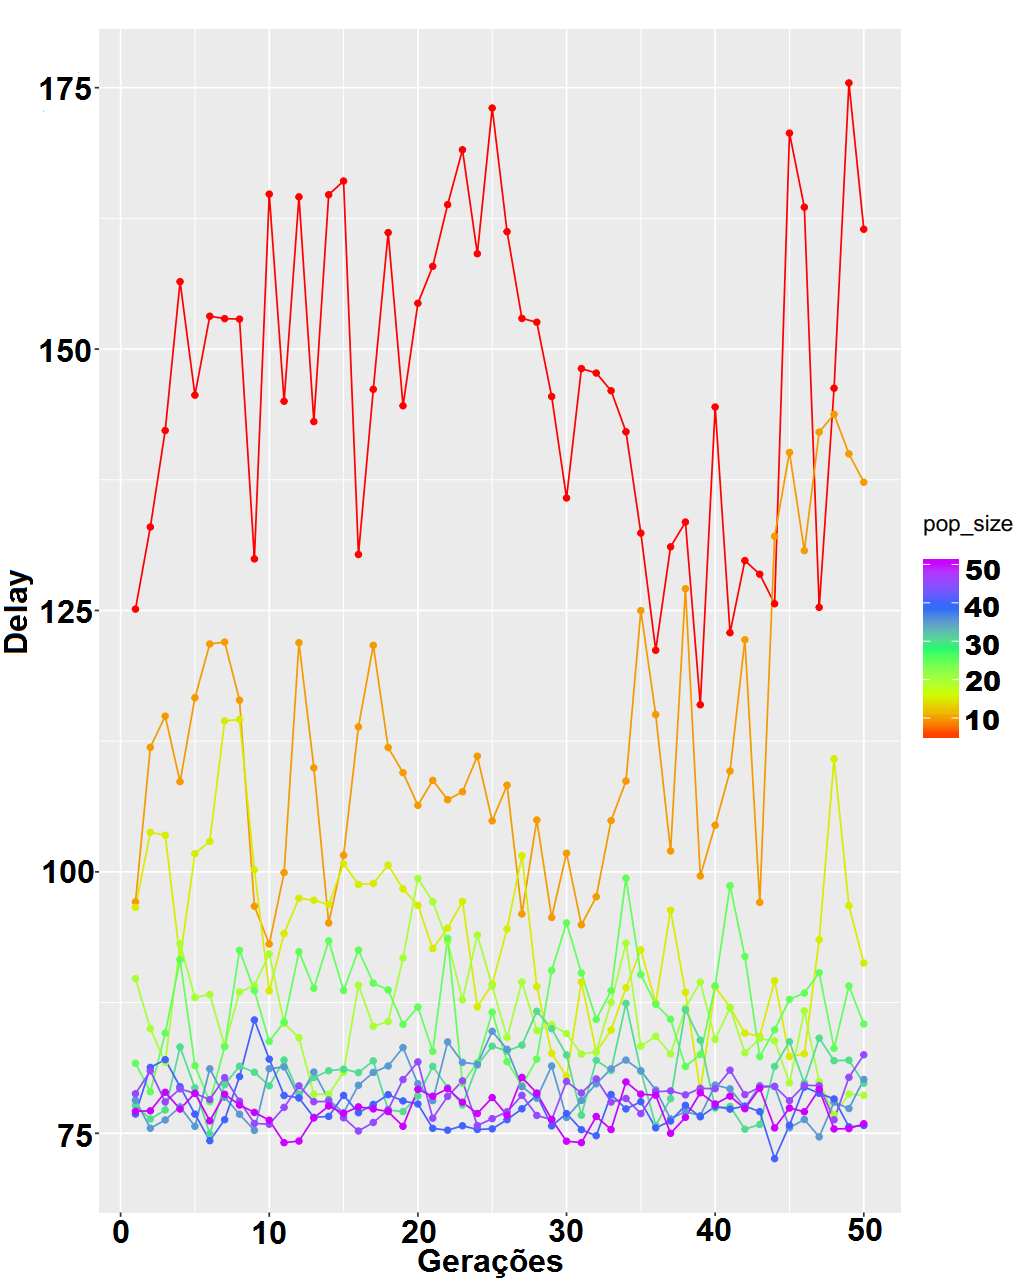
\includegraphics[scale=0.24]{figures/GeracoesXDelay.png}
  \caption{Resultado em termos de gerações por média de delay alcançados nas simulações.}
  \label{fig:result-delay}
\end{figure}


\subsection{Simulações por Geração}

Com a população variando de 5 a 50 indivíduos, o número de simulações aumenta proporcionalmente ao número de indivíduos e gerações, como pode ser observado na figura ~\ref{fig:result-sim}. Observa-se que o número de simulações chega a pouco menos de 2500 para uma população de 50 indivíduos, consistindo em um alto número de simulações para obter resultados ótimos se comparado a poucos indivíduos.

\begin{figure}[t]
  \centering
  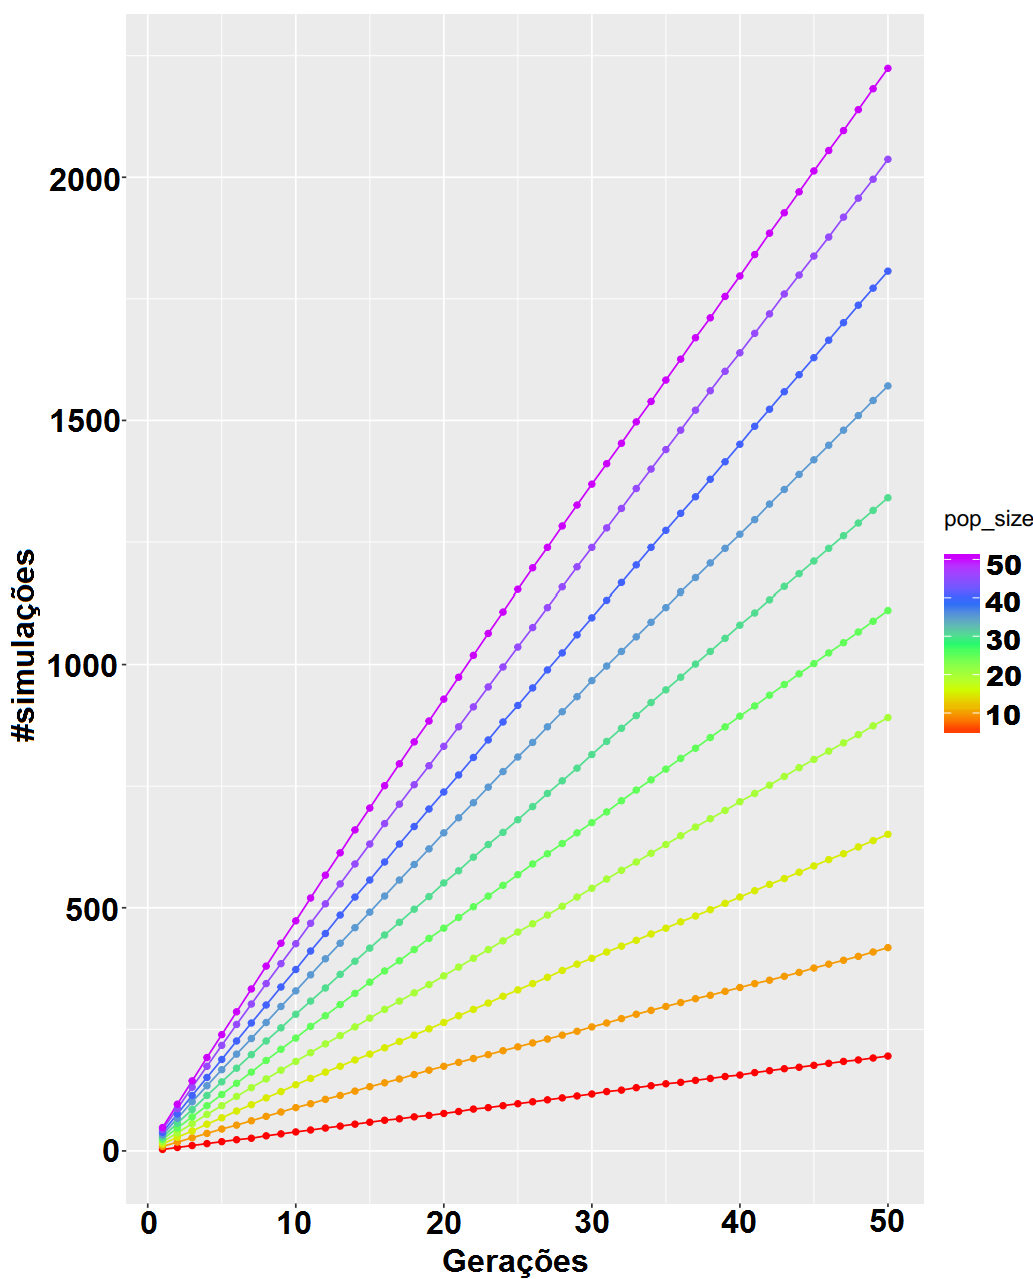
\includegraphics[scale=0.24]{figures/SimulacoesPorGeracao.png}
  \caption{Número de simulações por geração.}
  \label{fig:result-sim}
\end{figure}

\subsection{Comparação com exaustivo}

Os resultados da simulação exaustiva para os cenários propostos neste trabalho podem ser comparados com o pareto ótimo dos resultados obtidos com o algoritmo NSGA-II. As figuras ~\ref{fig:exaustivo-nsgaii-1},~\ref{fig:exaustivo-nsgaii-2} e ~\ref{fig:exaustivo-nsgaii-3}.

\begin{figure}[h]
  \centering
  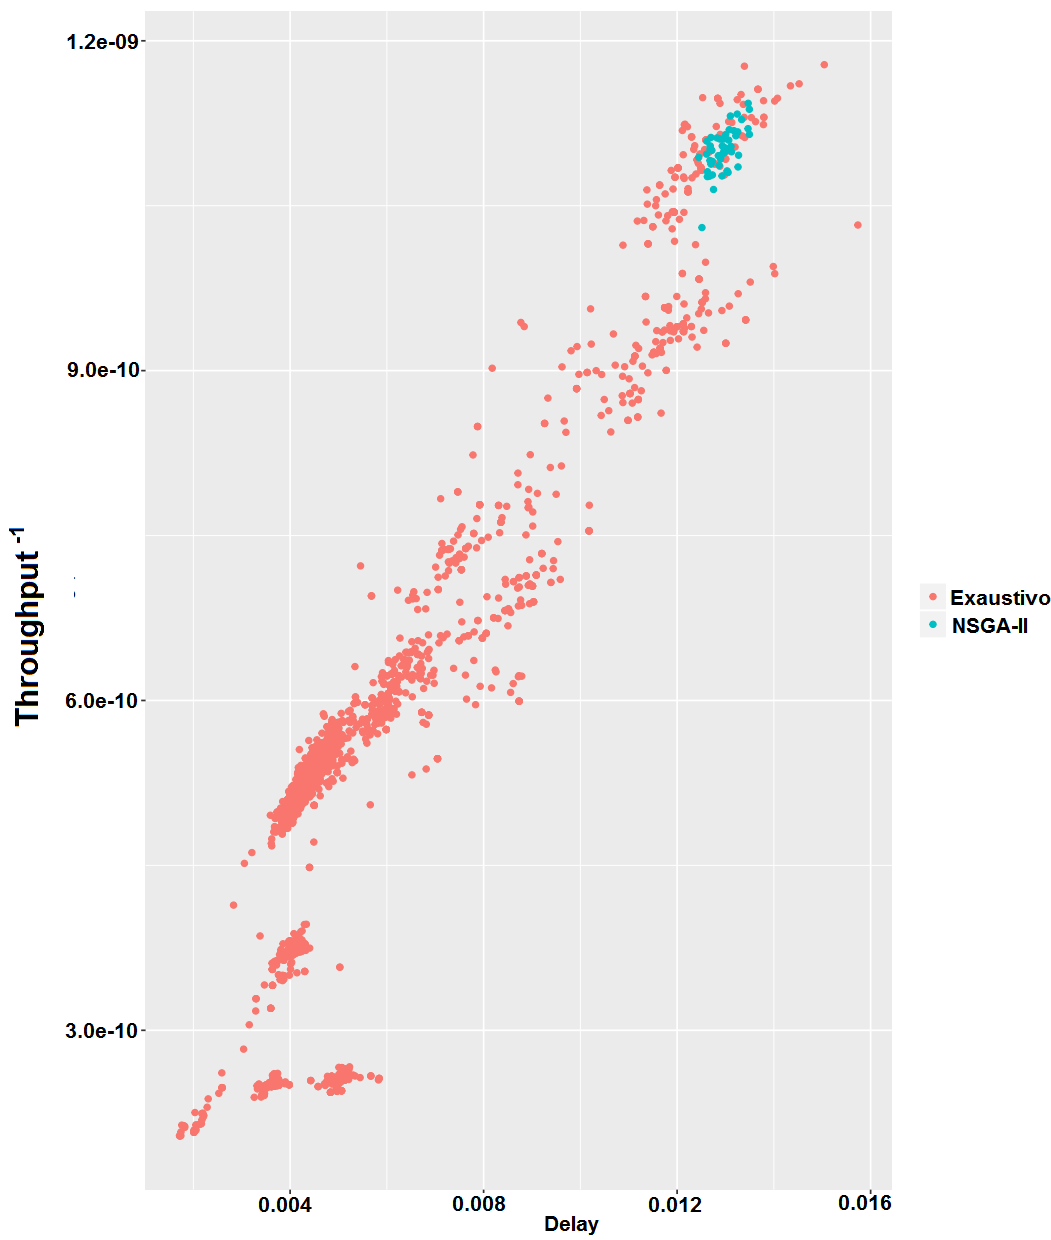
\includegraphics[scale=0.27]{figures/ExaustivoXNsgaii_DelayXThroughput.png}
  \caption{Comparação entre a simulação exaustiva e o NSGA-II em termos de Delay X Throughput.}
  \label{fig:exaustivo-nsgaii-1}
\end{figure}


\begin{figure}[h]
  \centering
  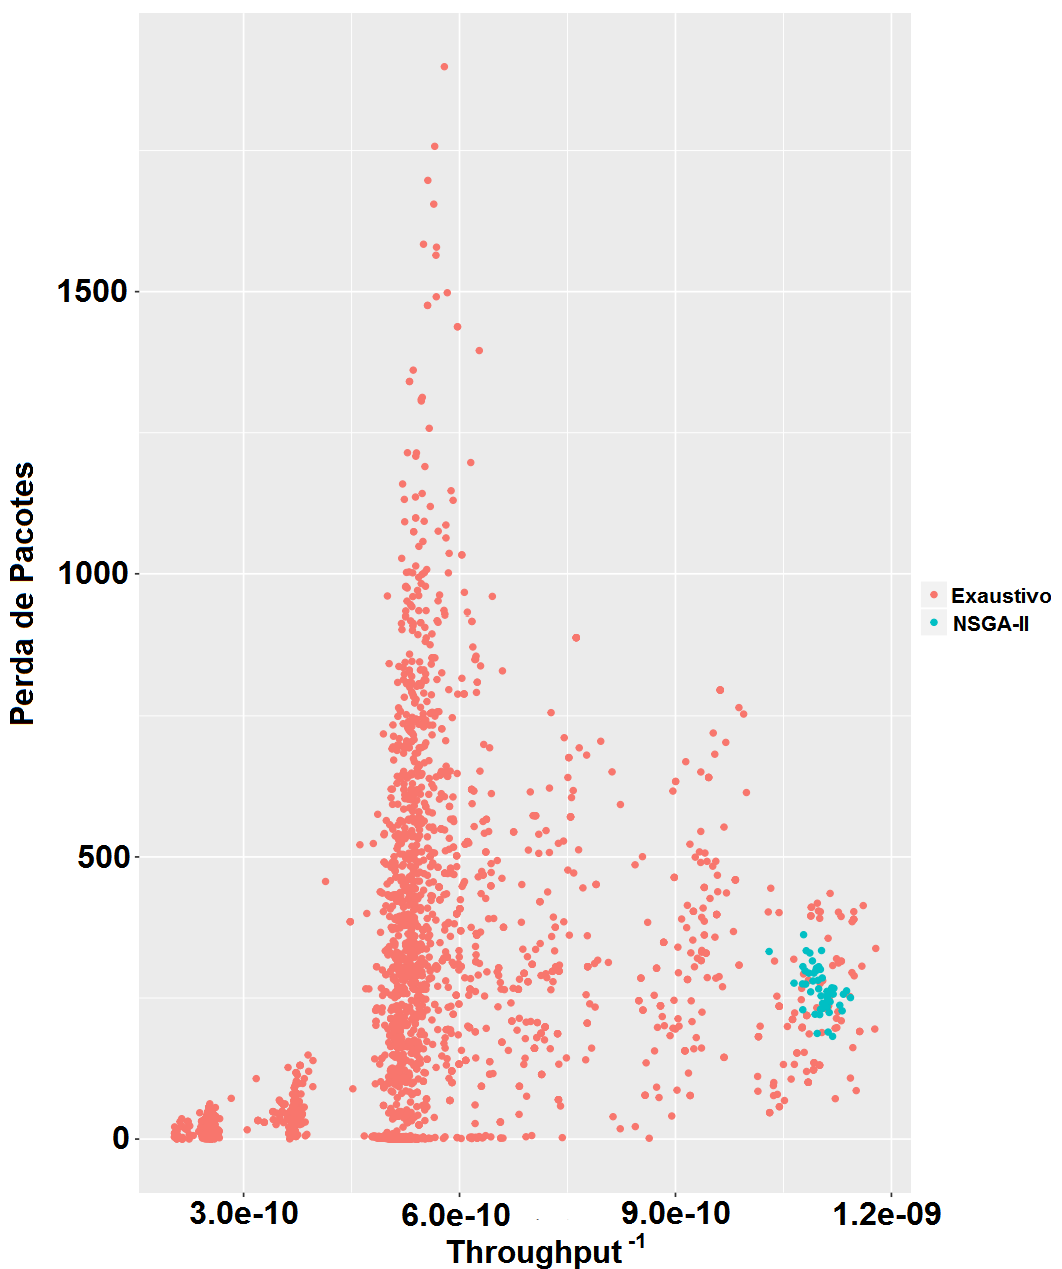
\includegraphics[scale=0.27]{figures/ExaustivoXNsgaii_ThroughputXPerdaPacotes.png}
  \caption{Comparação entre a simulação exaustiva e o NSGA-II em termos de Throughput X Perda de Pacotes.}
  \label{fig:exaustivo-nsgaii-2}
\end{figure}


\begin{figure}[h]
  \centering
  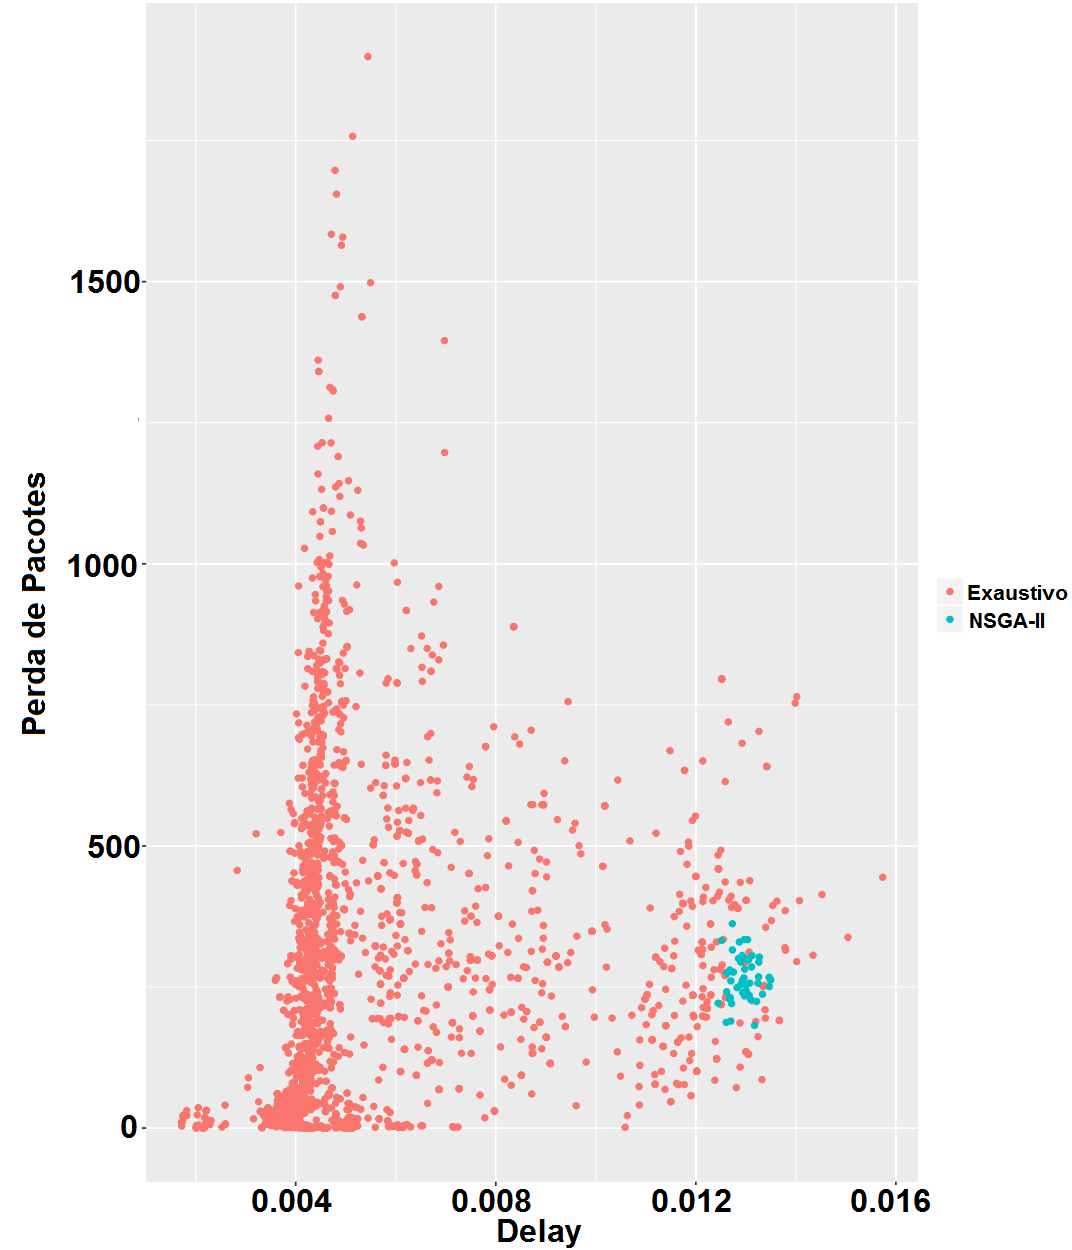
\includegraphics[scale=0.27]{figures/ExaustivoXNsgaii_DelayXPerdaPacotes.png}
  \caption{Comparação entre a simulação exaustiva e o NSGA-II em termos de Delay X Perda de Pacotes.}
  \label{fig:exaustivo-nsgaii-3}
\end{figure}



\section{Conclusão}

Neste trabalho, foi apresentada uma implementação do algoritmo NSGA-II como forma de otimizar e alcançar configurações ótimas visando minimizar o número de simulações a serem executadas com o intuito de (1) minimizar a perda de pacotes, (2) minimizar o delay e (3) maximizar o throughput na comunicação V2V num cenário urbano real.  Os resultados mostraram que é possível obter uma rápida convergência de soluções ótimas com poucas gerações se considerada uma população de 40 a 50 indivíduos. No entanto, é visível o alto número de simulações necessários para obter chegar a tal conclusão, chegando a pouco mais de 2000 simulações. Para trabalhos futuros, sugere-se a implementação de outras técnicas multiobjetivas com o intuito de avaliar a mais eficiente para este caso.


%\nocite{*} % Include everything in the .bib file.

\bibliographystyle{IEEEtran}
\bibliography{bibl}

% that's all, folks
\end{document}
